Second-order moving average (MA2) is a probabilistic model commonly
used for time series analysis. The observation at time $t$ is given
by:

\begin{gather} \label{eq:ma2}
y_t = w_t + \theta_1 w_{t-1} + \theta_2 w_{t-2}\\
\theta_1, \theta_2 \in \R, \quad  w_k \sim \mathcal{N}(0,1), k \in \mathbb{Z}
\end{gather}

\noindent
The random variable $w_{k} \sim \mathcal{N}(0,1), k \in \mathbb{Z}$
represent white noise and $\theta_1, \theta_2$, the two parameters of
interest, the dependence from the previous observations. The number of
consecutive observations $T$ is a hyper-parameter of the model that in
our case is set at $T=100$. For guaranteeing that the inference
problem is identifiable, i.e.\ the likelihood has only one mode, we
use the prior proposed by \cite{Marin2012} given in the equation
\eqref{eq:ma2_prior}:

\begin{equation} \label{eq:ma2_prior}
p(\thetab) = p(\theta_1)p(\theta_2|\theta_1)
= \mathcal{U}(\theta_1;-2,2)\mathcal{U}(\theta_2;\theta_1-1, \theta_1+1)
\end{equation}

% \begin{figure}[ht]
%     \begin{center}
%       \includegraphics[width=0.48\textwidth]{./latex_files/images/chapter4/mae2_prior_samples.png}
%     \end{center}
%     \caption[MA2 example, prior distribution.]{Prior distribution proposed by \cite{Marin2012}. The
%       samples follow a triangular shape.}
%   \label{fig:ma2_1}
% \end{figure}

\noindent
The observation vector $\yb_0 = (y_1, \ldots, y_{100})$ is generated
with $\thetab^*=(0.6, 0.2)$. The dimensionality of the output $\yb$ is
high, therefore we use summary statistics. Considering that the
ouptput vector represents a time-series signal, we choose as summary
statistics the autocovariances with $lag=1$ and $lag=2$, as shown in
equations \eqref{eq:ma2_summary_1} and \eqref{eq:ma2_summary_2}. The
final distance node is the squared euclidean
distance \eqref{eq:ma2_summary_4}.

\begin{gather} \label{eq:ma2_summary_1}
  s_1(\yb) = \frac{1}{T-1} \sum_{t=2}^T y_ty_{t-1}\\ \label{eq:ma2_summary_2}
  s_2(\yb) = \frac{1}{T-2} \sum_{t=3}^T y_ty_{t-2} \\
  s(\yb) = (s_1(\yb), s_2(\yb))\\ \label{eq:ma2_summary_4}
  d = ||s(\yb) - s(\yb_0)||_2^2 
\end{gather}

\subsubsection*{Perform the inference}

As in the previous example, we perform the inference using both
optimisation alternatives (gradient-based and Bayesian optimisation)
and we compare the results at each step. In the end, we use the
Rejection ABC algorithm for evaluating both approximations. Rejection
ABC is a robust method in terms of accuracy and can be used for
baseline comparison.

In figure \ref{fig:ma2_5}, we illustrate the acceptance region of the
same deterministic simulator, i.e. with \code{seed=799981517}, in the
gradient-based and the Bayesian optimisation case. The acceptance
regions are similar in both cases. The optimal points are close and
the search directions are similar. This indicates that both
optimization scemes work robustly. Therefore, we observe that as we
move away from the optimal pint, the surrogate model fitted by the
Bayesian Optimisation tends to deviate from the real distance. This
divergence affects the bounding box approximation and explains some
small differences between the posterior approximations, as shown in
figure \ref{fig:ma2_3}. In figure \ref{fig:ma2_3}, we demonstrate the
histograms of the marginal posteriors, using the three different
methods; (a) Rejection ABC (first line), (b) ROMC with gradient-based
optimisation (second line) and (c) ROMC with Bayesian optimisation
(third line). Undoubtedly, we observe that there is a significant
similarity between the three approaches. The Rejection ABC inference
has been set to infer 10000 accepted samples, with threshold
$\epsilon=0.1$. At table \ref{tab:ma2} we present the empirical mean
$\mu$ and standard deviation $\sigma$ for each inference approach, for
verifying their agreement.

\begin{center} \label{tab:ma2}
\begin{tabular}{ c|c|c|c|c }
\hline
& $\mu_{\theta_1}$ & $\sigma_{\theta_1}$ & $\mu_{\theta_2}$ & $\sigma_{\theta_2}$ \\
\hline \hline
Rejection ABC & 0.516 & 0.142 & 0.07 & 0.172 \\
\hline
ROMC (gradient-based) & 0.504 & 0.143 & 0.033 & 0.171 \\
\hline
ROMC (Bayesian optimisation) & 0.502 & 0.166 & 0.079 & 0.168 \\
\hline
\end{tabular}
\end{center}

% \begin{figure}[H]
%     \begin{center}
%       \includegraphics[width=0.48\textwidth]{./latex_files/images/chapter4/ma2_distance_hist.png}
%       \includegraphics[width=0.48\textwidth]{./latex_files/images/chapter4/ma2_distance_hist_bo.png} \\
%     \end{center}
%     \caption[MA2 example, histogram of distances]{Histogram of distances
%       $d_i^*, i \in \{ 1, \ldots, n_1 \}$. The left graph corresponds
%       to the gradient-based approach and the right one to the Bayesian
%       optimisation approach.}
%   \label{fig:ma2_2}
% \end{figure}

\begin{figure}[ht]
    \begin{center}
        % \input{./latex_files/images/chapter4/ma2_region_3.tex}
        % \input{./latex_files/images/chapter4/ma2_region_3_bo.tex}
        \includegraphics[width=0.49\textwidth]{./latex_files/images/chapter4/ma2_region_1.png}
        \includegraphics[width=0.49\textwidth]{./latex_files/images/chapter4/ma2_region_1_bo.png}
    \end{center}
  \caption[The acceptance region of a specific deterministic simulator.]{The acceptance region in a specific optimisation problem. In the left figure the region obtained with gradient-based optimiser and in the right one with Bayesian Optimisation.}
  \label{fig:ma2_5}
\end{figure}


% \begin{figure}[h]
%     \begin{center}
%       \includegraphics[width=0.35\textwidth]{./latex_files/images/chapter4/mae2_hist_t1_rejection.png}
%       \includegraphics[width=0.35\textwidth]{./latex_files/images/chapter4/mae2_hist_t2_rejection.png}\\
%       \includegraphics[width=0.35\textwidth]{./latex_files/images/chapter4/mae2_hist_t1_romc.png}
%       \includegraphics[width=0.35\textwidth]{./latex_files/images/chapter4/mae2_hist_t2_romc.png}\\
%       \includegraphics[width=0.35\textwidth]{./latex_files/images/chapter4/mae2_hist_t1_romc_bo.png}
%       \includegraphics[width=0.35\textwidth]{./latex_files/images/chapter4/mae2_hist_t2_romc_bo.png}\\
%     \end{center}
%     \caption[MA2 example, evaluation of the marginal
%     distributions.]{Histogram of the marginal posterior distributions
%       using three different inference approaches; (a) in the first
%       row, the samples are obtained using Rejection ABC sampling (b)
%       in the second row, using ROMC with a gradient-based optimiser
%       and (c) in the third row, using ROMC with Bayesian optimization
%       approach. The vertical (red) line represents the samples mean
%       $\mu$ and the horizontal (black) the standard deviation
%       $\sigma$.}
%   \label{fig:ma2_3}
% \end{figure}


\begin{figure}[ht]
  \begin{center}
    \input{./latex_files/images/chapter4/mae2_hist_t1_rejection.tex}
    \input{./latex_files/images/chapter4/mae2_hist_t2_rejection.tex}\\
    % This file was created with tikzplotlib v0.9.12.
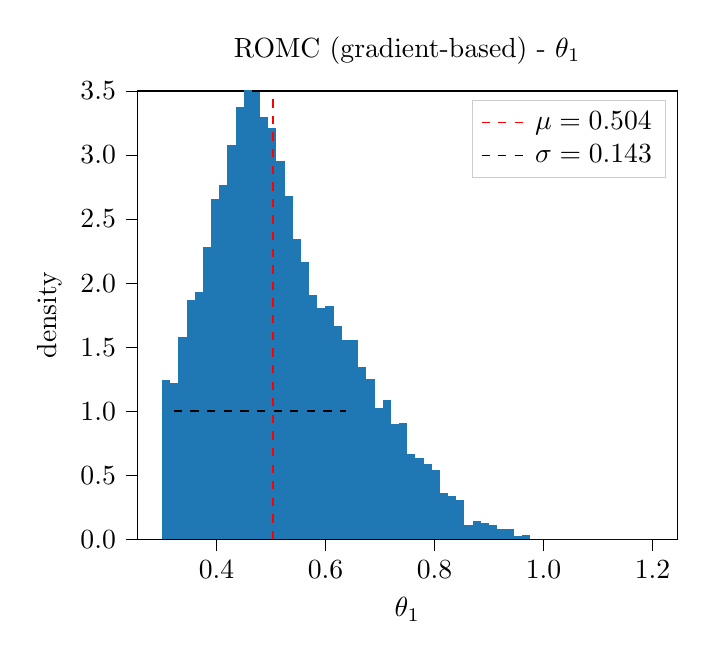
\begin{tikzpicture}

\definecolor{color0}{rgb}{0.12156862745098,0.466666666666667,0.705882352941177}

\begin{axis}[
legend cell align={left},
legend style={fill opacity=0.8, draw opacity=1, text opacity=1, draw=white!80!black},
tick align=outside,
tick pos=left,
title={ROMC (gradient-based) - \(\displaystyle \theta_1\)},
x grid style={white!69.0196078431373!black},
xlabel={\(\displaystyle \theta_1\)},
xmin=0.255, xmax=1.245,
xtick style={color=black},
xtick={0.2,0.4,0.6,0.8,1,1.2,1.4},
xticklabels={
  \(\displaystyle {0.2}\),
  \(\displaystyle {0.4}\),
  \(\displaystyle {0.6}\),
  \(\displaystyle {0.8}\),
  \(\displaystyle {1.0}\),
  \(\displaystyle {1.2}\),
  \(\displaystyle {1.4}\)
},
y grid style={white!69.0196078431373!black},
ylabel={density},
ymin=0, ymax=3.5,
ytick style={color=black},
ytick={0,0.5,1,1.5,2,2.5,3,3.5},
yticklabels={
  \(\displaystyle {0.0}\),
  \(\displaystyle {0.5}\),
  \(\displaystyle {1.0}\),
  \(\displaystyle {1.5}\),
  \(\displaystyle {2.0}\),
  \(\displaystyle {2.5}\),
  \(\displaystyle {3.0}\),
  \(\displaystyle {3.5}\)
}
]
\draw[draw=none,fill=color0] (axis cs:0.3,0) rectangle (axis cs:0.315,1.23969307221967);
\draw[draw=none,fill=color0] (axis cs:0.315,0) rectangle (axis cs:0.33,1.22260605418476);
\draw[draw=none,fill=color0] (axis cs:0.33,0) rectangle (axis cs:0.345,1.58099417689925);
\draw[draw=none,fill=color0] (axis cs:0.345,0) rectangle (axis cs:0.36,1.86697039022021);
\draw[draw=none,fill=color0] (axis cs:0.36,0) rectangle (axis cs:0.375,1.9327905830084);
\draw[draw=none,fill=color0] (axis cs:0.375,0) rectangle (axis cs:0.39,2.28560027755721);
\draw[draw=none,fill=color0] (axis cs:0.39,0) rectangle (axis cs:0.405,2.65528249842742);
\draw[draw=none,fill=color0] (axis cs:0.405,0) rectangle (axis cs:0.42,2.76542029517717);
\draw[draw=none,fill=color0] (axis cs:0.42,0) rectangle (axis cs:0.435,3.08006607906211);
\draw[draw=none,fill=color0] (axis cs:0.435,0) rectangle (axis cs:0.45,3.37496095644731);
\draw[draw=none,fill=color0] (axis cs:0.45,0) rectangle (axis cs:0.465,3.55021219168023);
\draw[draw=none,fill=color0] (axis cs:0.465,0) rectangle (axis cs:0.48,3.48979291667414);
\draw[draw=none,fill=color0] (axis cs:0.48,0) rectangle (axis cs:0.495,3.29497485978374);
\draw[draw=none,fill=color0] (axis cs:0.495,0) rectangle (axis cs:0.51,3.21369852560985);
\draw[draw=none,fill=color0] (axis cs:0.51,0) rectangle (axis cs:0.525,2.95263129250428);
\draw[draw=none,fill=color0] (axis cs:0.525,0) rectangle (axis cs:0.54,2.68186180204391);
\draw[draw=none,fill=color0] (axis cs:0.54,0) rectangle (axis cs:0.555,2.34177450679284);
\draw[draw=none,fill=color0] (axis cs:0.555,0) rectangle (axis cs:0.57,2.16665229531096);
\draw[draw=none,fill=color0] (axis cs:0.57,0) rectangle (axis cs:0.585,1.90550699050888);
\draw[draw=none,fill=color0] (axis cs:0.585,0) rectangle (axis cs:0.6,1.80681861350051);
\draw[draw=none,fill=color0] (axis cs:0.6,0) rectangle (axis cs:0.615,1.82068989944754);
\draw[draw=none,fill=color0] (axis cs:0.615,0) rectangle (axis cs:0.63,1.66308656575326);
\draw[draw=none,fill=color0] (axis cs:0.63,0) rectangle (axis cs:0.645,1.55350554347052);
\draw[draw=none,fill=color0] (axis cs:0.645,0) rectangle (axis cs:0.66,1.55706027108261);
\draw[draw=none,fill=color0] (axis cs:0.66,0) rectangle (axis cs:0.675,1.34606411506585);
\draw[draw=none,fill=color0] (axis cs:0.675,0) rectangle (axis cs:0.69,1.25058859381965);
\draw[draw=none,fill=color0] (axis cs:0.69,0) rectangle (axis cs:0.705,1.02541420681756);
\draw[draw=none,fill=color0] (axis cs:0.705,0) rectangle (axis cs:0.72,1.08883061316133);
\draw[draw=none,fill=color0] (axis cs:0.72,0) rectangle (axis cs:0.735,0.901026681844632);
\draw[draw=none,fill=color0] (axis cs:0.735,0) rectangle (axis cs:0.75,0.90959073604536);
\draw[draw=none,fill=color0] (axis cs:0.75,0) rectangle (axis cs:0.765,0.663388353950532);
\draw[draw=none,fill=color0] (axis cs:0.765,0) rectangle (axis cs:0.78,0.635304321110202);
\draw[draw=none,fill=color0] (axis cs:0.78,0) rectangle (axis cs:0.795,0.584894248497155);
\draw[draw=none,fill=color0] (axis cs:0.795,0) rectangle (axis cs:0.81,0.541909616027169);
\draw[draw=none,fill=color0] (axis cs:0.81,0) rectangle (axis cs:0.825,0.364723435432413);
\draw[draw=none,fill=color0] (axis cs:0.825,0) rectangle (axis cs:0.84,0.337243430980688);
\draw[draw=none,fill=color0] (axis cs:0.84,0) rectangle (axis cs:0.855,0.304888876342628);
\draw[draw=none,fill=color0] (axis cs:0.855,0) rectangle (axis cs:0.87,0.11082071864216);
\draw[draw=none,fill=color0] (axis cs:0.87,0) rectangle (axis cs:0.885,0.14353193766205);
\draw[draw=none,fill=color0] (axis cs:0.885,0) rectangle (axis cs:0.9,0.12562311229572);
\draw[draw=none,fill=color0] (axis cs:0.9,0) rectangle (axis cs:0.915,0.107714286929387);
\draw[draw=none,fill=color0] (axis cs:0.915,0) rectangle (axis cs:0.93,0.0820282878821482);
\draw[draw=none,fill=color0] (axis cs:0.93,0) rectangle (axis cs:0.945,0.0827149079075519);
\draw[draw=none,fill=color0] (axis cs:0.945,0) rectangle (axis cs:0.96,0.0269285717323464);
\draw[draw=none,fill=color0] (axis cs:0.96,0) rectangle (axis cs:0.975,0.0307869571533697);
\draw[draw=none,fill=color0] (axis cs:0.975,0) rectangle (axis cs:0.99,0);
\draw[draw=none,fill=color0] (axis cs:0.99,0) rectangle (axis cs:1.005,0);
\draw[draw=none,fill=color0] (axis cs:1.005,0) rectangle (axis cs:1.02,0);
\draw[draw=none,fill=color0] (axis cs:1.02,0) rectangle (axis cs:1.035,0);
\draw[draw=none,fill=color0] (axis cs:1.035,0) rectangle (axis cs:1.05,0);
\draw[draw=none,fill=color0] (axis cs:1.05,0) rectangle (axis cs:1.065,0);
\draw[draw=none,fill=color0] (axis cs:1.065,0) rectangle (axis cs:1.08,0);
\draw[draw=none,fill=color0] (axis cs:1.08,0) rectangle (axis cs:1.095,0);
\draw[draw=none,fill=color0] (axis cs:1.095,0) rectangle (axis cs:1.11,0);
\draw[draw=none,fill=color0] (axis cs:1.11,0) rectangle (axis cs:1.125,0);
\draw[draw=none,fill=color0] (axis cs:1.125,0) rectangle (axis cs:1.14,0);
\draw[draw=none,fill=color0] (axis cs:1.14,0) rectangle (axis cs:1.155,0);
\draw[draw=none,fill=color0] (axis cs:1.155,0) rectangle (axis cs:1.17,0);
\draw[draw=none,fill=color0] (axis cs:1.17,0) rectangle (axis cs:1.185,0);
\draw[draw=none,fill=color0] (axis cs:1.185,0) rectangle (axis cs:1.2,0);
\addplot [semithick, red, dashed]
table {%
0.50403516578119 0
0.50403516578119 3.5
};
\addlegendentry{$\mu = 0.504$}
\addplot [semithick, black, dashed]
table {%
0.321847690178847 1
0.637029674539771 1
};
\addlegendentry{$\sigma = 0.143$}
\end{axis}

\end{tikzpicture}

    % This file was created with tikzplotlib v0.9.12.
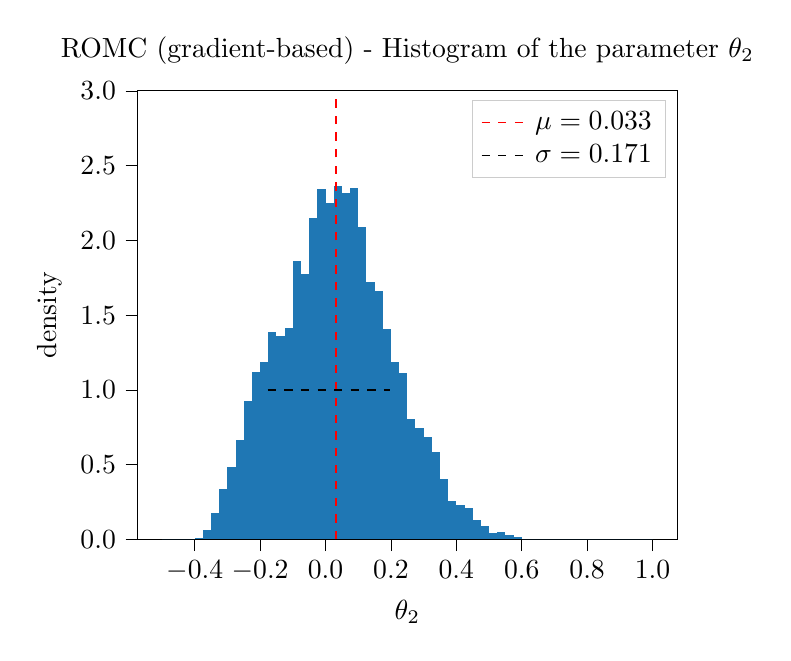
\begin{tikzpicture}

\definecolor{color0}{rgb}{0.12156862745098,0.466666666666667,0.705882352941177}

\begin{axis}[
legend cell align={left},
legend style={fill opacity=0.8, draw opacity=1, text opacity=1, draw=white!80!black},
tick align=outside,
tick pos=left,
title={ROMC (gradient-based) - Histogram of the parameter \(\displaystyle \theta_2\)},
x grid style={white!69.0196078431373!black},
xlabel={\(\displaystyle \theta_2\)},
xmin=-0.575, xmax=1.075,
xtick style={color=black},
xtick={-0.6,-0.4,-0.2,0,0.2,0.4,0.6,0.8,1,1.2},
xticklabels={
  \(\displaystyle {\ensuremath{-}0.6}\),
  \(\displaystyle {\ensuremath{-}0.4}\),
  \(\displaystyle {\ensuremath{-}0.2}\),
  \(\displaystyle {0.0}\),
  \(\displaystyle {0.2}\),
  \(\displaystyle {0.4}\),
  \(\displaystyle {0.6}\),
  \(\displaystyle {0.8}\),
  \(\displaystyle {1.0}\),
  \(\displaystyle {1.2}\)
},
y grid style={white!69.0196078431373!black},
ylabel={density},
ymin=0, ymax=3,
ytick style={color=black},
ytick={0,0.5,1,1.5,2,2.5,3},
yticklabels={
  \(\displaystyle {0.0}\),
  \(\displaystyle {0.5}\),
  \(\displaystyle {1.0}\),
  \(\displaystyle {1.5}\),
  \(\displaystyle {2.0}\),
  \(\displaystyle {2.5}\),
  \(\displaystyle {3.0}\)
}
]
\draw[draw=none,fill=color0] (axis cs:-0.5,0) rectangle (axis cs:-0.475,0);
\draw[draw=none,fill=color0] (axis cs:-0.475,0) rectangle (axis cs:-0.45,0);
\draw[draw=none,fill=color0] (axis cs:-0.45,0) rectangle (axis cs:-0.425,0);
\draw[draw=none,fill=color0] (axis cs:-0.425,0) rectangle (axis cs:-0.4,0);
\draw[draw=none,fill=color0] (axis cs:-0.4,0) rectangle (axis cs:-0.375,0.00554428884192465);
\draw[draw=none,fill=color0] (axis cs:-0.375,0) rectangle (axis cs:-0.35,0.0609051679887177);
\draw[draw=none,fill=color0] (axis cs:-0.35,0) rectangle (axis cs:-0.325,0.172932144280507);
\draw[draw=none,fill=color0] (axis cs:-0.325,0) rectangle (axis cs:-0.3,0.33874934889258);
\draw[draw=none,fill=color0] (axis cs:-0.3,0) rectangle (axis cs:-0.275,0.484235646321314);
\draw[draw=none,fill=color0] (axis cs:-0.275,0) rectangle (axis cs:-0.25,0.665208164482786);
\draw[draw=none,fill=color0] (axis cs:-0.25,0) rectangle (axis cs:-0.225,0.92463814505837);
\draw[draw=none,fill=color0] (axis cs:-0.225,0) rectangle (axis cs:-0.2,1.12139409849263);
\draw[draw=none,fill=color0] (axis cs:-0.2,0) rectangle (axis cs:-0.175,1.18629739177248);
\draw[draw=none,fill=color0] (axis cs:-0.175,0) rectangle (axis cs:-0.15,1.38911741112759);
\draw[draw=none,fill=color0] (axis cs:-0.15,0) rectangle (axis cs:-0.125,1.3586665597235);
\draw[draw=none,fill=color0] (axis cs:-0.125,0) rectangle (axis cs:-0.1,1.4168730451184);
\draw[draw=none,fill=color0] (axis cs:-0.1,0) rectangle (axis cs:-0.075,1.86440804043856);
\draw[draw=none,fill=color0] (axis cs:-0.075,0) rectangle (axis cs:-0.05,1.77193230571172);
\draw[draw=none,fill=color0] (axis cs:-0.05,0) rectangle (axis cs:-0.025,2.14800442101592);
\draw[draw=none,fill=color0] (axis cs:-0.025,0) rectangle (axis cs:0,2.34373098482187);
\draw[draw=none,fill=color0] (axis cs:0,0) rectangle (axis cs:0.025,2.24893542723874);
\draw[draw=none,fill=color0] (axis cs:0.025,0) rectangle (axis cs:0.05,2.36527262608105);
\draw[draw=none,fill=color0] (axis cs:0.05,0) rectangle (axis cs:0.0750000000000001,2.32011000423491);
\draw[draw=none,fill=color0] (axis cs:0.0750000000000001,0) rectangle (axis cs:0.1,2.35112752816106);
\draw[draw=none,fill=color0] (axis cs:0.1,0) rectangle (axis cs:0.125,2.09237672296862);
\draw[draw=none,fill=color0] (axis cs:0.125,0) rectangle (axis cs:0.15,1.72225524667604);
\draw[draw=none,fill=color0] (axis cs:0.15,0) rectangle (axis cs:0.175,1.65885907591305);
\draw[draw=none,fill=color0] (axis cs:0.175,0) rectangle (axis cs:0.2,1.4089028988961);
\draw[draw=none,fill=color0] (axis cs:0.2,0) rectangle (axis cs:0.225,1.18892677075576);
\draw[draw=none,fill=color0] (axis cs:0.225,0) rectangle (axis cs:0.25,1.11057927007035);
\draw[draw=none,fill=color0] (axis cs:0.25,0) rectangle (axis cs:0.275,0.808010795099994);
\draw[draw=none,fill=color0] (axis cs:0.275,0) rectangle (axis cs:0.3,0.746145310081448);
\draw[draw=none,fill=color0] (axis cs:0.3,0) rectangle (axis cs:0.325,0.68232985247479);
\draw[draw=none,fill=color0] (axis cs:0.325,0) rectangle (axis cs:0.35,0.586634734027065);
\draw[draw=none,fill=color0] (axis cs:0.35,0) rectangle (axis cs:0.375,0.400470451389202);
\draw[draw=none,fill=color0] (axis cs:0.375,0) rectangle (axis cs:0.4,0.259104715630191);
\draw[draw=none,fill=color0] (axis cs:0.4,0) rectangle (axis cs:0.425,0.230773630659991);
\draw[draw=none,fill=color0] (axis cs:0.425,0) rectangle (axis cs:0.45,0.211235556781049);
\draw[draw=none,fill=color0] (axis cs:0.45,0) rectangle (axis cs:0.475,0.129869421833243);
\draw[draw=none,fill=color0] (axis cs:0.475,0) rectangle (axis cs:0.5,0.0903839207491964);
\draw[draw=none,fill=color0] (axis cs:0.5,0) rectangle (axis cs:0.525,0.0434117816322698);
\draw[draw=none,fill=color0] (axis cs:0.525,0) rectangle (axis cs:0.55,0.0482353129247447);
\draw[draw=none,fill=color0] (axis cs:0.55,0) rectangle (axis cs:0.575,0.0289411877548468);
\draw[draw=none,fill=color0] (axis cs:0.575,0) rectangle (axis cs:0.6,0.0144705938774233);
\draw[draw=none,fill=color0] (axis cs:0.6,0) rectangle (axis cs:0.625,0);
\draw[draw=none,fill=color0] (axis cs:0.625,0) rectangle (axis cs:0.65,0);
\draw[draw=none,fill=color0] (axis cs:0.65,0) rectangle (axis cs:0.675,0);
\draw[draw=none,fill=color0] (axis cs:0.675,0) rectangle (axis cs:0.7,0);
\draw[draw=none,fill=color0] (axis cs:0.7,0) rectangle (axis cs:0.725,0);
\draw[draw=none,fill=color0] (axis cs:0.725,0) rectangle (axis cs:0.75,0);
\draw[draw=none,fill=color0] (axis cs:0.75,0) rectangle (axis cs:0.775,0);
\draw[draw=none,fill=color0] (axis cs:0.775,0) rectangle (axis cs:0.8,0);
\draw[draw=none,fill=color0] (axis cs:0.8,0) rectangle (axis cs:0.825,0);
\draw[draw=none,fill=color0] (axis cs:0.825,0) rectangle (axis cs:0.85,0);
\draw[draw=none,fill=color0] (axis cs:0.85,0) rectangle (axis cs:0.875,0);
\draw[draw=none,fill=color0] (axis cs:0.875,0) rectangle (axis cs:0.9,0);
\draw[draw=none,fill=color0] (axis cs:0.9,0) rectangle (axis cs:0.925,0);
\draw[draw=none,fill=color0] (axis cs:0.925,0) rectangle (axis cs:0.95,0);
\draw[draw=none,fill=color0] (axis cs:0.95,0) rectangle (axis cs:0.975,0);
\draw[draw=none,fill=color0] (axis cs:0.975,0) rectangle (axis cs:1,0);
\addplot [semithick, red, dashed]
table {%
0.0325607299281219 0
0.0325607299281219 3
};
\addlegendentry{$\mu = 0.033$}
\addplot [semithick, black, dashed]
table {%
-0.17677281465975 1
0.198406420501618 1
};
\addlegendentry{$\sigma = 0.171$}
\end{axis}

\end{tikzpicture}
\\
    % This file was created with tikzplotlib v0.9.12.
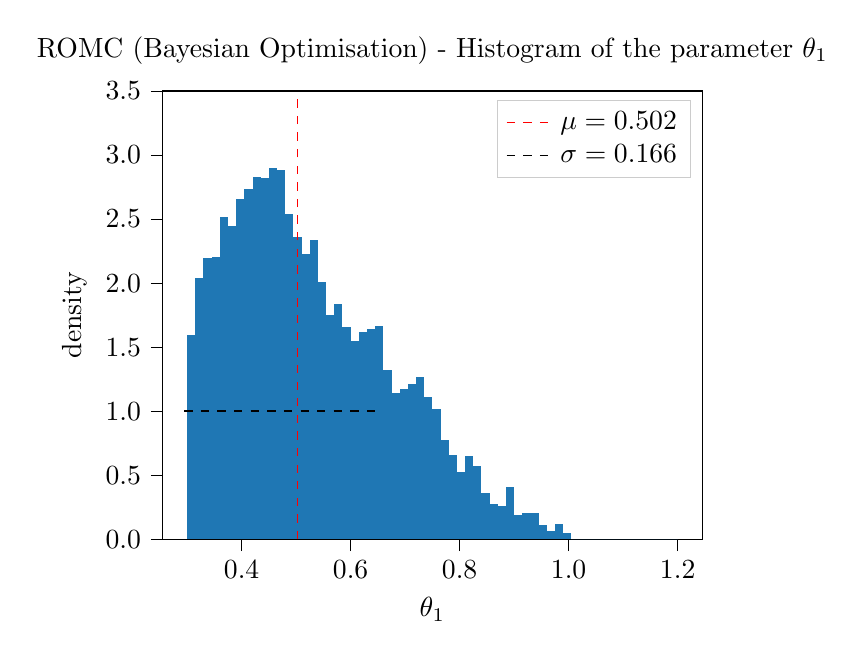
\begin{tikzpicture}

\definecolor{color0}{rgb}{0.12156862745098,0.466666666666667,0.705882352941177}

\begin{axis}[
legend cell align={left},
legend style={fill opacity=0.8, draw opacity=1, text opacity=1, draw=white!80!black},
tick align=outside,
tick pos=left,
title={ROMC (Bayesian Optimisation) - Histogram of the parameter \(\displaystyle \theta_1\)},
x grid style={white!69.0196078431373!black},
xlabel={\(\displaystyle \theta_1\)},
xmin=0.255, xmax=1.245,
xtick style={color=black},
xtick={0.2,0.4,0.6,0.8,1,1.2,1.4},
xticklabels={
  \(\displaystyle {0.2}\),
  \(\displaystyle {0.4}\),
  \(\displaystyle {0.6}\),
  \(\displaystyle {0.8}\),
  \(\displaystyle {1.0}\),
  \(\displaystyle {1.2}\),
  \(\displaystyle {1.4}\)
},
y grid style={white!69.0196078431373!black},
ylabel={density},
ymin=0, ymax=3.5,
ytick style={color=black},
ytick={0,0.5,1,1.5,2,2.5,3,3.5},
yticklabels={
  \(\displaystyle {0.0}\),
  \(\displaystyle {0.5}\),
  \(\displaystyle {1.0}\),
  \(\displaystyle {1.5}\),
  \(\displaystyle {2.0}\),
  \(\displaystyle {2.5}\),
  \(\displaystyle {3.0}\),
  \(\displaystyle {3.5}\)
}
]
\draw[draw=none,fill=color0] (axis cs:0.3,0) rectangle (axis cs:0.315,1.59230812208571);
\draw[draw=none,fill=color0] (axis cs:0.315,0) rectangle (axis cs:0.33,2.04310565145056);
\draw[draw=none,fill=color0] (axis cs:0.33,0) rectangle (axis cs:0.345,2.19382815490065);
\draw[draw=none,fill=color0] (axis cs:0.345,0) rectangle (axis cs:0.36,2.20021699441589);
\draw[draw=none,fill=color0] (axis cs:0.36,0) rectangle (axis cs:0.375,2.51506116421806);
\draw[draw=none,fill=color0] (axis cs:0.375,0) rectangle (axis cs:0.39,2.44880980882892);
\draw[draw=none,fill=color0] (axis cs:0.39,0) rectangle (axis cs:0.405,2.65904829491329);
\draw[draw=none,fill=color0] (axis cs:0.405,0) rectangle (axis cs:0.42,2.73250343027527);
\draw[draw=none,fill=color0] (axis cs:0.42,0) rectangle (axis cs:0.435,2.82852250487442);
\draw[draw=none,fill=color0] (axis cs:0.435,0) rectangle (axis cs:0.45,2.82331312648089);
\draw[draw=none,fill=color0] (axis cs:0.45,0) rectangle (axis cs:0.465,2.90135211837164);
\draw[draw=none,fill=color0] (axis cs:0.465,0) rectangle (axis cs:0.48,2.88136478592358);
\draw[draw=none,fill=color0] (axis cs:0.48,0) rectangle (axis cs:0.495,2.53560317010369);
\draw[draw=none,fill=color0] (axis cs:0.495,0) rectangle (axis cs:0.51,2.3564598017404);
\draw[draw=none,fill=color0] (axis cs:0.51,0) rectangle (axis cs:0.525,2.22420707945385);
\draw[draw=none,fill=color0] (axis cs:0.525,0) rectangle (axis cs:0.54,2.33534256536061);
\draw[draw=none,fill=color0] (axis cs:0.54,0) rectangle (axis cs:0.555,2.00495652659749);
\draw[draw=none,fill=color0] (axis cs:0.555,0) rectangle (axis cs:0.57,1.74992091039568);
\draw[draw=none,fill=color0] (axis cs:0.57,0) rectangle (axis cs:0.585,1.83870977452066);
\draw[draw=none,fill=color0] (axis cs:0.585,0) rectangle (axis cs:0.6,1.6578788920657);
\draw[draw=none,fill=color0] (axis cs:0.6,0) rectangle (axis cs:0.615,1.55026416918985);
\draw[draw=none,fill=color0] (axis cs:0.615,0) rectangle (axis cs:0.63,1.62152961093496);
\draw[draw=none,fill=color0] (axis cs:0.63,0) rectangle (axis cs:0.645,1.6437730803435);
\draw[draw=none,fill=color0] (axis cs:0.645,0) rectangle (axis cs:0.66,1.66640493128548);
\draw[draw=none,fill=color0] (axis cs:0.66,0) rectangle (axis cs:0.675,1.32365272171391);
\draw[draw=none,fill=color0] (axis cs:0.675,0) rectangle (axis cs:0.69,1.14155317519524);
\draw[draw=none,fill=color0] (axis cs:0.69,0) rectangle (axis cs:0.705,1.17480604967746);
\draw[draw=none,fill=color0] (axis cs:0.705,0) rectangle (axis cs:0.72,1.20896637137188);
\draw[draw=none,fill=color0] (axis cs:0.72,0) rectangle (axis cs:0.735,1.26617555858479);
\draw[draw=none,fill=color0] (axis cs:0.735,0) rectangle (axis cs:0.75,1.10815016078187);
\draw[draw=none,fill=color0] (axis cs:0.75,0) rectangle (axis cs:0.765,1.01575133068398);
\draw[draw=none,fill=color0] (axis cs:0.765,0) rectangle (axis cs:0.78,0.778653581806476);
\draw[draw=none,fill=color0] (axis cs:0.78,0) rectangle (axis cs:0.795,0.658517776017212);
\draw[draw=none,fill=color0] (axis cs:0.795,0) rectangle (axis cs:0.81,0.522857721601219);
\draw[draw=none,fill=color0] (axis cs:0.81,0) rectangle (axis cs:0.825,0.649384569447495);
\draw[draw=none,fill=color0] (axis cs:0.825,0) rectangle (axis cs:0.84,0.571069158563703);
\draw[draw=none,fill=color0] (axis cs:0.84,0) rectangle (axis cs:0.855,0.362376122626364);
\draw[draw=none,fill=color0] (axis cs:0.855,0) rectangle (axis cs:0.87,0.275087556542002);
\draw[draw=none,fill=color0] (axis cs:0.87,0) rectangle (axis cs:0.885,0.255847252846728);
\draw[draw=none,fill=color0] (axis cs:0.885,0) rectangle (axis cs:0.9,0.406941618766892);
\draw[draw=none,fill=color0] (axis cs:0.9,0) rectangle (axis cs:0.915,0.192257669195406);
\draw[draw=none,fill=color0] (axis cs:0.915,0) rectangle (axis cs:0.93,0.204927790769102);
\draw[draw=none,fill=color0] (axis cs:0.93,0) rectangle (axis cs:0.945,0.203525138747285);
\draw[draw=none,fill=color0] (axis cs:0.945,0) rectangle (axis cs:0.96,0.113584712363094);
\draw[draw=none,fill=color0] (axis cs:0.96,0) rectangle (axis cs:0.975,0.0662010640185658);
\draw[draw=none,fill=color0] (axis cs:0.975,0) rectangle (axis cs:0.99,0.116253091726246);
\draw[draw=none,fill=color0] (axis cs:0.99,0) rectangle (axis cs:1.005,0.0456418048890116);
\draw[draw=none,fill=color0] (axis cs:1.005,0) rectangle (axis cs:1.02,0);
\draw[draw=none,fill=color0] (axis cs:1.02,0) rectangle (axis cs:1.035,0);
\draw[draw=none,fill=color0] (axis cs:1.035,0) rectangle (axis cs:1.05,0);
\draw[draw=none,fill=color0] (axis cs:1.05,0) rectangle (axis cs:1.065,0);
\draw[draw=none,fill=color0] (axis cs:1.065,0) rectangle (axis cs:1.08,0);
\draw[draw=none,fill=color0] (axis cs:1.08,0) rectangle (axis cs:1.095,0);
\draw[draw=none,fill=color0] (axis cs:1.095,0) rectangle (axis cs:1.11,0);
\draw[draw=none,fill=color0] (axis cs:1.11,0) rectangle (axis cs:1.125,0);
\draw[draw=none,fill=color0] (axis cs:1.125,0) rectangle (axis cs:1.14,0);
\draw[draw=none,fill=color0] (axis cs:1.14,0) rectangle (axis cs:1.155,0);
\draw[draw=none,fill=color0] (axis cs:1.155,0) rectangle (axis cs:1.17,0);
\draw[draw=none,fill=color0] (axis cs:1.17,0) rectangle (axis cs:1.185,0);
\draw[draw=none,fill=color0] (axis cs:1.185,0) rectangle (axis cs:1.2,0);
\addplot [semithick, red, dashed]
table {%
0.502312841390367 0
0.502312841390367 3.5
};
\addlegendentry{$\mu = 0.502$}
\addplot [semithick, black, dashed]
table {%
0.294820390999603 1
0.660267860059204 1
};
\addlegendentry{$\sigma = 0.166$}
\end{axis}

\end{tikzpicture}

    % This file was created with tikzplotlib v0.9.12.
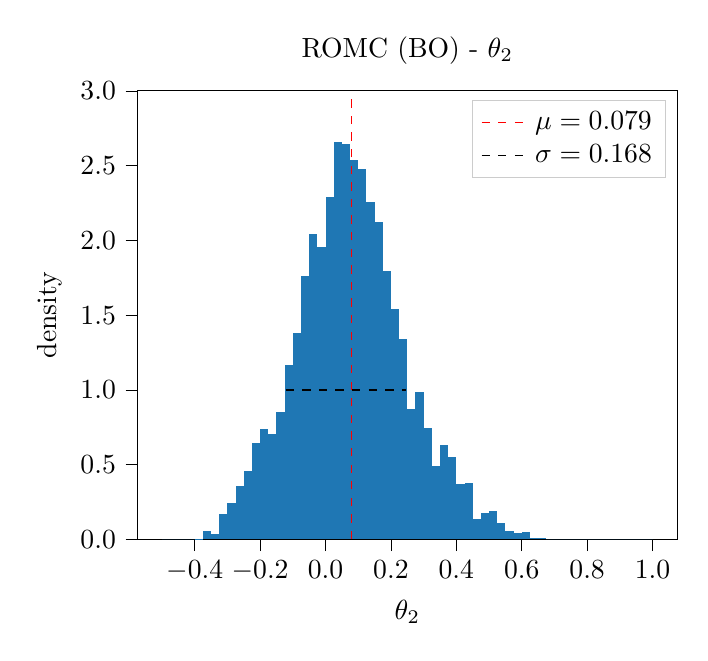
\begin{tikzpicture}

\definecolor{color0}{rgb}{0.12156862745098,0.466666666666667,0.705882352941177}

\begin{axis}[
legend cell align={left},
legend style={fill opacity=0.8, draw opacity=1, text opacity=1, draw=white!80!black},
tick align=outside,
tick pos=left,
title={ROMC (BO) - \(\displaystyle \theta_2\)},
x grid style={white!69.0196078431373!black},
xlabel={\(\displaystyle \theta_2\)},
xmin=-0.575, xmax=1.075,
xtick style={color=black},
xtick={-0.6,-0.4,-0.2,0,0.2,0.4,0.6,0.8,1,1.2},
xticklabels={
  \(\displaystyle {\ensuremath{-}0.6}\),
  \(\displaystyle {\ensuremath{-}0.4}\),
  \(\displaystyle {\ensuremath{-}0.2}\),
  \(\displaystyle {0.0}\),
  \(\displaystyle {0.2}\),
  \(\displaystyle {0.4}\),
  \(\displaystyle {0.6}\),
  \(\displaystyle {0.8}\),
  \(\displaystyle {1.0}\),
  \(\displaystyle {1.2}\)
},
y grid style={white!69.0196078431373!black},
ylabel={density},
ymin=0, ymax=3,
ytick style={color=black},
ytick={0,0.5,1,1.5,2,2.5,3},
yticklabels={
  \(\displaystyle {0.0}\),
  \(\displaystyle {0.5}\),
  \(\displaystyle {1.0}\),
  \(\displaystyle {1.5}\),
  \(\displaystyle {2.0}\),
  \(\displaystyle {2.5}\),
  \(\displaystyle {3.0}\)
}
]
\draw[draw=none,fill=color0] (axis cs:-0.5,0) rectangle (axis cs:-0.475,0);
\draw[draw=none,fill=color0] (axis cs:-0.475,0) rectangle (axis cs:-0.45,0);
\draw[draw=none,fill=color0] (axis cs:-0.45,0) rectangle (axis cs:-0.425,0);
\draw[draw=none,fill=color0] (axis cs:-0.425,0) rectangle (axis cs:-0.4,0);
\draw[draw=none,fill=color0] (axis cs:-0.4,0) rectangle (axis cs:-0.375,0.00425643655908195);
\draw[draw=none,fill=color0] (axis cs:-0.375,0) rectangle (axis cs:-0.35,0.0584436505421199);
\draw[draw=none,fill=color0] (axis cs:-0.35,0) rectangle (axis cs:-0.325,0.032329412084104);
\draw[draw=none,fill=color0] (axis cs:-0.325,0) rectangle (axis cs:-0.3,0.170488346927624);
\draw[draw=none,fill=color0] (axis cs:-0.3,0) rectangle (axis cs:-0.275,0.241312187040701);
\draw[draw=none,fill=color0] (axis cs:-0.275,0) rectangle (axis cs:-0.25,0.353203225767864);
\draw[draw=none,fill=color0] (axis cs:-0.25,0) rectangle (axis cs:-0.225,0.454783676389647);
\draw[draw=none,fill=color0] (axis cs:-0.225,0) rectangle (axis cs:-0.2,0.645870310110015);
\draw[draw=none,fill=color0] (axis cs:-0.2,0) rectangle (axis cs:-0.175,0.736855945766172);
\draw[draw=none,fill=color0] (axis cs:-0.175,0) rectangle (axis cs:-0.15,0.7054880882772);
\draw[draw=none,fill=color0] (axis cs:-0.15,0) rectangle (axis cs:-0.125,0.853720954547648);
\draw[draw=none,fill=color0] (axis cs:-0.125,0) rectangle (axis cs:-0.1,1.16488627133908);
\draw[draw=none,fill=color0] (axis cs:-0.1,0) rectangle (axis cs:-0.075,1.37944888929298);
\draw[draw=none,fill=color0] (axis cs:-0.075,0) rectangle (axis cs:-0.05,1.75863459008645);
\draw[draw=none,fill=color0] (axis cs:-0.05,0) rectangle (axis cs:-0.025,2.04186645728356);
\draw[draw=none,fill=color0] (axis cs:-0.025,0) rectangle (axis cs:0,1.95487930439736);
\draw[draw=none,fill=color0] (axis cs:0,0) rectangle (axis cs:0.025,2.2931926651875);
\draw[draw=none,fill=color0] (axis cs:0.025,0) rectangle (axis cs:0.05,2.65546746491156);
\draw[draw=none,fill=color0] (axis cs:0.05,0) rectangle (axis cs:0.0750000000000001,2.64247045528465);
\draw[draw=none,fill=color0] (axis cs:0.0750000000000001,0) rectangle (axis cs:0.1,2.53538619434107);
\draw[draw=none,fill=color0] (axis cs:0.1,0) rectangle (axis cs:0.125,2.47437216167486);
\draw[draw=none,fill=color0] (axis cs:0.125,0) rectangle (axis cs:0.15,2.25894133814364);
\draw[draw=none,fill=color0] (axis cs:0.15,0) rectangle (axis cs:0.175,2.12306099510411);
\draw[draw=none,fill=color0] (axis cs:0.175,0) rectangle (axis cs:0.2,1.79209215192117);
\draw[draw=none,fill=color0] (axis cs:0.2,0) rectangle (axis cs:0.225,1.53877177811189);
\draw[draw=none,fill=color0] (axis cs:0.225,0) rectangle (axis cs:0.25,1.34176813031492);
\draw[draw=none,fill=color0] (axis cs:0.25,0) rectangle (axis cs:0.275,0.869256102075021);
\draw[draw=none,fill=color0] (axis cs:0.275,0) rectangle (axis cs:0.3,0.984211536278622);
\draw[draw=none,fill=color0] (axis cs:0.3,0) rectangle (axis cs:0.325,0.744495637346589);
\draw[draw=none,fill=color0] (axis cs:0.325,0) rectangle (axis cs:0.35,0.487332826886714);
\draw[draw=none,fill=color0] (axis cs:0.35,0) rectangle (axis cs:0.375,0.631223471040121);
\draw[draw=none,fill=color0] (axis cs:0.375,0) rectangle (axis cs:0.4,0.5510631368371);
\draw[draw=none,fill=color0] (axis cs:0.4,0) rectangle (axis cs:0.425,0.369415701030125);
\draw[draw=none,fill=color0] (axis cs:0.425,0) rectangle (axis cs:0.45,0.376101401475276);
\draw[draw=none,fill=color0] (axis cs:0.45,0) rectangle (axis cs:0.475,0.135239439335051);
\draw[draw=none,fill=color0] (axis cs:0.475,0) rectangle (axis cs:0.5,0.17253048109158);
\draw[draw=none,fill=color0] (axis cs:0.5,0) rectangle (axis cs:0.525,0.187926500765093);
\draw[draw=none,fill=color0] (axis cs:0.525,0) rectangle (axis cs:0.55,0.106413103399642);
\draw[draw=none,fill=color0] (axis cs:0.55,0) rectangle (axis cs:0.575,0.0572991796412681);
\draw[draw=none,fill=color0] (axis cs:0.575,0) rectangle (axis cs:0.6,0.0435129826888125);
\draw[draw=none,fill=color0] (axis cs:0.6,0) rectangle (axis cs:0.625,0.0491139237583741);
\draw[draw=none,fill=color0] (axis cs:0.625,0) rectangle (axis cs:0.65,0.011416843630065);
\draw[draw=none,fill=color0] (axis cs:0.65,0) rectangle (axis cs:0.675,0.0114168436300651);
\draw[draw=none,fill=color0] (axis cs:0.675,0) rectangle (axis cs:0.7,3.98076835078974e-05);
\draw[draw=none,fill=color0] (axis cs:0.7,0) rectangle (axis cs:0.725,0);
\draw[draw=none,fill=color0] (axis cs:0.725,0) rectangle (axis cs:0.75,0);
\draw[draw=none,fill=color0] (axis cs:0.75,0) rectangle (axis cs:0.775,0);
\draw[draw=none,fill=color0] (axis cs:0.775,0) rectangle (axis cs:0.8,0);
\draw[draw=none,fill=color0] (axis cs:0.8,0) rectangle (axis cs:0.825,0);
\draw[draw=none,fill=color0] (axis cs:0.825,0) rectangle (axis cs:0.85,0);
\draw[draw=none,fill=color0] (axis cs:0.85,0) rectangle (axis cs:0.875,0);
\draw[draw=none,fill=color0] (axis cs:0.875,0) rectangle (axis cs:0.9,0);
\draw[draw=none,fill=color0] (axis cs:0.9,0) rectangle (axis cs:0.925,0);
\draw[draw=none,fill=color0] (axis cs:0.925,0) rectangle (axis cs:0.95,0);
\draw[draw=none,fill=color0] (axis cs:0.95,0) rectangle (axis cs:0.975,0);
\draw[draw=none,fill=color0] (axis cs:0.975,0) rectangle (axis cs:1,0);
\addplot [semithick, red, dashed]
table {%
0.0793529734576715 0
0.0793529734576715 3
};
\addlegendentry{$\mu = 0.079$}
\addplot [semithick, black, dashed]
table {%
-0.122023559466631 1
0.246600101073509 1
};
\addlegendentry{$\sigma = 0.168$}
\end{axis}

\end{tikzpicture}
\\
    \end{center}
    \caption[MA2 example, evaluation of the marginal
    distributions.]{Histogram of the marginal posterior distributions
      using three different inference approaches; (a) in the first
      row, the samples are obtained using Rejection ABC sampling (b)
      in the second row, using ROMC with a gradient-based optimiser
      and (c) in the third row, using ROMC with Bayesian optimization
      approach. The vertical (red) line represents the samples mean
      $\mu$ and the horizontal (black) the standard deviation
      $\sigma$.}
  \label{fig:ma2_3}
\end{figure}



% \begin{figure}[H]
%     \begin{center}
%       \includegraphics[width=0.48\textwidth]{./latex_files/images/chapter4/mae2_romc_posterior.png}
%       \includegraphics[width=0.48\textwidth]{./latex_files/images/chapter4/mae2_romc_posterior_bo.png}
%     \end{center}
%     \caption[MA2 example, approximate posterior.]{ROMC approximate posteriors using gradient-based approach
%       (left) and Bayesian optimisation approach (right).}
%   \label{fig:ma2_4}
% \end{figure}

